
%%%%%%%%%%%%%%%%%%%%%%%%%%%%%%%%%%%%%%%%%%%%%%%%%%%%%%%%%%%%%%%%%%%%%%%%%%%%%%%%%%%%%%%
\section{Diode Clipper Modeling}
\label{chap:diode_clipper}
%%%%%%%%%%%%%%%%%%%%%%%%%%%%%%%%%%%%%%%%%%%%%%%%%%%%%%%%%%%%%%%%%%%%%%%%%%%%%%%%%%%%%%%

This section presents the results of diode clipper modeling. First, the training data used for training and evaluation is discussed. Second, the training procedure is outlined. Third, the models themselves are listed with their hyperparameters. Finally, the obtained results are compared.

%%%%%%%%%%%%%%%%%%%%%%%%%%%%%%%%%%%%%%%%%%%%%%%%%%%%%%%%%%%%%%%%%%%%%%%%%%%%%%%%%%%%%%%
\subsection{Training Data}
\label{sec:diode_clipper_training_data}
%%%%%%%%%%%%%%%%%%%%%%%%%%%%%%%%%%%%%%%%%%%%%%%%%%%%%%%%%%%%%%%%%%%%%%%%%%%%%%%%%%%%%%%

The dataset used for diode clipper modeling consisted of 7 minutes and 59 seconds of guitar and bass recordings from \cite{Abesser2013} and \cite{Kehling2014} respectively. The amount of guitar recordings was roughly the same as the amount of bass recordings and their ordering was arbitrary. All recordings were single-channel and used \SI{44100}{Hz} sampling rate. Out of these, 1 minute and 29 seconds (approximately 20\%) were used as the test set. 

Care was taken so that the test file begins with silence. Thanks to this, ODENet's initialization with the all-zero vector did not obscure the comparison between the architectures in terms of quality. If the first true output sample was far from zero, the all-zero initialization would cause a click in ODENet's test output. 

The remaining data was split into the validation set (1 minute and 18 seconds) and the train set (5 minutes and 12 seconds) according to the 80:20 rule. The input to the model was the raw recording. The target distorted signal was synthesized from a SPICE model of the circuit with the schematic from \Figure{fig:diode_clipper_circuit} and parameter values from \Table{tab:diode_clipper_element_parameters}. For the simulation, LTspice XVII by Analog Devices was used \cite{LTspice}. The synthesized target data sounds realistic.

%%%%%%%%%%%%%%%%%%%%%%%%%%%%%%%%%%%%%%%%%%%%%%%%%%%%%%%%%%%%%%%%%%%%%%%%%%%%%%%%%%%%%%%
\subsection{Training}
\label{sec:diode_clipper_training}
%%%%%%%%%%%%%%%%%%%%%%%%%%%%%%%%%%%%%%%%%%%%%%%%%%%%%%%%%%%%%%%%%%%%%%%%%%%%%%%%%%%%%%%

The training procedure was as follows. Firstly, the dataset was loaded, then the network architecture was initialized, and the training parameters were set (optimization algorithm, hyperparameters, learning rate schedule, loss function). Then the proper training was run for a fixed number of epochs. After each epoch, the validation loss was computed. Finally, after finishing the last epoch, the test set was processed and the model's output along with the final loss value were recorded.

The training set was split into half-second segments. These segments were randomly shuffled at the beginning of each epoch and grouped into minibatches of a predetermined size.

A single epoch consisted of processing the minibatches of segments in chunks (subsegments) of length equal to 2048 samples. At the beginning of each minibatch, \ac{LSTM}8 architecture processed 1000 samples of input to let the hidden states properly initialize. After each subsegment, the gradient of the loss with respect to the network parameters was calculated using the \ac{BPTT}. Then, a gradient step was performed using the Adam optimizer \cite{Kingma2017}, the computational graph was discarded, and the next subsegment was processed. After each minibatch, the learning rate scheduler performed its step (if such a scheduler was set). When an epoch ended, model parameters were stored by overwriting the previously saved ones. Additionally, the training session kept track of the model which performed best on the validation set.

The number of epochs in training was determined by manually observing the validation loss curve. If the validation loss reached a plateau below 1\% of the loss, the training was deemed successful.

%%%%%%%%%%%%%%%%%%%%%%%%%%%%%%%%%%%%%%%%%%%%%%%%%%%%%%%%%%%%%%%%%%%%%%%%%%%%%%%%%%%%%%%
\subsection{Compared Models}
\label{sec:diode_clipper_models}
%%%%%%%%%%%%%%%%%%%%%%%%%%%%%%%%%%%%%%%%%%%%%%%%%%%%%%%%%%%%%%%%%%%%%%%%%%%%%%%%%%%%%%%

For the assessment of how well ODENet can model the diode clipper, two derivative networks were chosen: $2 \times 100 \times 100 \times 1$ (ODENet100) and $2 \times 9 \times 9 \times 1$ (ODENet9), both with the \ac{ReLU} nonlinearity. The former was used to ensure that the network has enough capacity to learn the derivative of the diode clipper \ac{ODE}. The latter was the smallest derivative network that has reached validation loss smaller than 1\%. The goal of decreasing the size of the derivative network was to see what is the minimum feasible number of parameters that the network must have to successfully model the diode clipper. The smaller the network, the faster the processing, thus, small networks are desired for possible real time processing.

Both these derivative networks were trained and tested with the forward Euler scheme. Additionally, the smaller one was trained and tested with the implicit Adams scheme and \ac{SELU} nonlinearity to see if it improves with a more accurate solver despite its small size.

For benchmark, the following architectures were chosen:
\begin{itemize}
    \item \ac{STN} from \cite{Parker2019} of size $2 \times 4 \times 4 \times 4 \times 1$ with $\tanh$ nonlinearity and biases enabled only in the second layer, 
    \item \ac{RINN} from \cite{Ouala2019} with \ac{RK}4 integration parameters and time step fixed to 1 (\ac{RINN}4) using a bilinear block with 6 units in each fully connected layer (BB6), and 
    \item \ac{LSTM}-based architecture from \cite{Wright2019} with 8 hidden units and an $8 \times 1$ output \ac{MLP} mapping the hidden states to an output sample (\ac{LSTM}8).
\end{itemize}

Each model is listed with its number of parameters,
hyperparameter values during training, training time (in epochs and hours), and teacher forcing curriculum in \Table{tab:diode_clipper_models_data}. The curriculum descriptions mean the following: "never" does not use teacher forcing, "always" provides true output for each minibatch at each time step, "bernoulli" uses scheduled sampling, where the probability of using teacher forcing for a minibatch decreases with each epoch. If a binary sample drawn from the Bernoulli distribution determines that teacher forcing should be used for a given minibatch, then the previous true output is supplied at each time step of the processing of that minibatch.

\begin{table}[]
    \resizebox{\textwidth}{!}{%
\begin{tabular}{@{}|l|c|c|c|c|c|c|@{}}
\toprule
Model & LSTM8 & \makecell{STN\\3x4\\tanh} & \makecell{ODENet\\FE\\hidden100\\ReLU} & \makecell{ODENet\\FE\\hidden9\\ReLU} & \makecell{ODENet\\IA\\hidden9\\SELU} & \makecell{RINN4\\BB6} \\ \midrule
Number of   parameters & 361 & 48 & 10501 & 127 & 127 & 67 \\ \midrule
Learning rate & 0.001 & 0.001 & 0.001 & 0.001 & 0.001 & 0.001 \\ \midrule
Learning rate schedule & none & none & \makecell{one-cycle\\LR 0.02} & \makecell{one-cycle\\LR 0.02} & \makecell{cyclical\\LR 0.01} & \makecell{one-cycle\\LR 0.02} \\ \midrule
Epochs in training & 200 & 340 & 300 & 300 & 600 & 600 \\ \midrule
Hours in training & 1 & 49 & 8 & 10 & 75 & 24 \\ \midrule
Teacher forcing & never & bernoulli & always & always & always & never \\ \bottomrule
\end{tabular}%
}

    \caption{Compared network architectures for diode clipper modeling}
    \label{tab:diode_clipper_models_data}
\end{table}

All of the architectures were trained on audio data at \SI{44100}{Hz} sampling rate. Each of these models was tested on previously unseen data at \SI{44100}{Hz} (same as training data), \SI{22050}{Hz}, \SI{48000}{Hz}, and \SI{192000}{Hz} sampling rates. The goal of using various sampling rates at test time was to analyze the presence of aliasing in the output and inspect the accuracy of the models at sampling rates different than the one in training. 

During test, \ac{STN} and ODENet models were informed about the new value of the time step, whereas \ac{LSTM}8 and \ac{RINN}4 were not. \ac{LSTM} and \ac{RINN} architectures don't provide a tunable parameter for explicitly changing the time step; they rather learn the time step from data.

Test loss $\mathcal{E}(y, \hat{y})$ given by \Equation{eq:final_loss_function}, \ac{segSNR} given by \Equation{eq:seg_snr}, and \ac{PEAQ} described in \Section{subsec:va_evaluation}.
were calculated for each model and test sampling rate. The meaning of the \ac{PEAQ} scores was explained in \Table{tab:itu_impairment_scale}.

All models were tested on a one long sequence but the implicit Adams scheme consistently diverged in this test setting. Therefore, its tests were conducted using segments of 22050 samples which were concatenated afterwards.

%%%%%%%%%%%%%%%%%%%%%%%%%%%%%%%%%%%%%%%%%%%%%%%%%%%%%%%%%%%%%%%%%%%%%%%%%%%%%%%%%%%%%%%
\subsection{Results and Discussion}
\label{sec:diode_clipper_results}
%%%%%%%%%%%%%%%%%%%%%%%%%%%%%%%%%%%%%%%%%%%%%%%%%%%%%%%%%%%%%%%%%%%%%%%%%%%%%%%%%%%%%%%

In \Table{tab:diode_clipper_results} the test results of the compared models are shown. The loss and \ac{PEAQ} were rounded to two significant digits, whereas \ac{segSNR} was rounded to one decimal place. The best results are given in bold (lowest loss, highest \ac{segSNR} and \ac{PEAQ}). The models were separately evaluated in terms of the learned model quality (test sampling rate equal to training sampling rate) and performance at sampling rates different from the training sampling rate. 

\begin{table}[]
    \newcommand{\modelNameCellWidth}{1.8cm}
%     \resizebox{\textwidth}{!}{%
%     \begin{tabular}{@{}l|c|l|c|c|c|c|c|c|@{}}
%         \cmidrule(l){2-9}
%         & Model & Metric & LSTM8 & \makecell{STN\\3x4\\tanh} & \makecell{ODENet100\\(FE)\\ReLU} & \makecell{ODENet9\\(FE)\\ReLU} & \makecell{ODENet9\\(IA)\\SELU} & \makecell{RINN4\\BB6} \\ \midrule
%         \multicolumn{1}{|c|}{\multirow{12}{*}{\rotatebox[origin=c]{270}{\hspace{1cm}test sampling rate [Hz]}}} & \multirow{3}{*}{ \makecell{44100\\(train)}} & 
%                                     Loss    & \textbf{0.041\%} & 0.45\% & 0.090\% & 0.37\% & 0.11\% & 0.19\% \\
%         \multicolumn{1}{|l|}{} &  & segSNR  & \textbf{30.5} & 18.5 & 25.3 & 23.4 & 24.6 & 25.0 \\
%         \multicolumn{1}{|l|}{} &  & ODG     & \textbf{-1.9} & -3.3 & -2.8 & -2.7 & -3.8 & -2.8 \\  \cmidrule(l){2-9}
%         \multicolumn{1}{|l|}{} & \multirow{3}{*}{22050} & 
%                                     Loss    & 0.71\% & 230\% & 530\% & 28\% & 63\% & \textbf{0.54\%} \\
%         \multicolumn{1}{|l|}{} &  & segSNR &  \textbf{24.0} & 5.1 & -5.7 & 10.9 & 2.5 & 23.9 \\
%         \multicolumn{1}{|l|}{} &  & ODG     & \textbf{-1.0} & -3.9 & -3.3 & -3.9 & -3.8 & -1.7 \\ \cmidrule(l){2-9}
%         \multicolumn{1}{|l|}{} & \multirow{3}{*}{48000} & 
%                                     Loss    & \textbf{0.042\%} & 0.37\% & 0.080\% & 0.34\% & 0.094\% & 0.18\% \\
%         \multicolumn{1}{|l|}{} &  & segSNR  & \textbf{30.0} & 18.9 & 25.9 & 23.7 & 24.8 & 25.0 \\
%         \multicolumn{1}{|l|}{} &  & ODG     & \textbf{-1.8} & -3.2 & -2.8 & -2.3 & -3.8 & -2.7 \\ \cmidrule(l){2-9}
%         \multicolumn{1}{|l|}{} & \multirow{3}{*}{192000} & 
%                                     Loss    & 0.55\% & 0.36\% & \textbf{0.070\%} & 0.22\% & 0.086\% & 0.56\% \\
%         \multicolumn{1}{|l|}{} &  & segSNR  & 21.6 & 19.0 & \textbf{28.4} & 25.9 & 24.7 & 20.6 \\
%         \multicolumn{1}{|l|}{} &  & ODG     & -3.6 & -3.2 & \textbf{-2.2} & -2.4 & -3.8 & -3.6 \\ \bottomrule
%     \end{tabular}%
%     }
    \resizebox{\textwidth}{!}{%
    \begin{tabular}{@{}l c l | c c c c c c @{}}
        \cmidrule(l){2-9}
        & \makecell{Test\\sampling\\rate [Hz]} & Model & LSTM8 & \makecell{STN\\3x4\\tanh} & \makecell{ODENet100\\(FE)\\ReLU} & \makecell{ODENet9\\(FE)\\ReLU} & \makecell{ODENet9\\(IA)\\SELU} & \makecell{RINN4\\BB6} \\ \midrule
        % & Test sampling rate [Hz] & Metric &  &  &  &  &  & \\ \midrule
        & \multirow{3}{*}{ \makecell{44100\\(train)}} & 
                                    Loss    & \textbf{0.041\%} & 0.45\% & 0.090\% & 0.37\% & 0.11\% & 0.19\% \\
        &  & segSNR  & \textbf{30.5} & 18.5 & 25.3 & 23.4 & 24.6 & 25.0 \\
        &  & ODG     & \textbf{-1.9} & -3.3 & -2.8 & -2.7 & -3.8 & -2.8 \\  \cmidrule(l){2-9}
        & \multirow{3}{*}{22050} & 
                                    Loss    & 0.71\% & 230\% & 530\% & 28\% & 63\% & \textbf{0.54\%} \\
        &  & segSNR &  \textbf{24.0} & 5.1 & -5.7 & 10.9 & 2.5 & 23.9 \\
        &  & ODG     & \textbf{-1.0} & -3.9 & -3.3 & -3.9 & -3.8 & -1.7 \\ \cmidrule(l){2-9}
        & \multirow{3}{*}{48000} & 
                                    Loss    & \textbf{0.042\%} & 0.37\% & 0.080\% & 0.34\% & 0.094\% & 0.18\% \\
        &  & segSNR  & \textbf{30.0} & 18.9 & 25.9 & 23.7 & 24.8 & 25.0 \\
        &  & ODG     & \textbf{-1.8} & -3.2 & -2.8 & -2.3 & -3.8 & -2.7 \\ \cmidrule(l){2-9}
        & \multirow{3}{*}{192000} & 
                                    Loss    & 0.55\% & 0.36\% & \textbf{0.070\%} & 0.22\% & 0.086\% & 0.56\% \\
        &  & segSNR  & 21.6 & 19.0 & \textbf{28.4} & 25.9 & 24.7 & 20.6 \\
        &  & ODG     & -3.6 & -3.2 & \textbf{-2.2} & -2.4 & -3.8 & -3.6 \\ \bottomrule
    \end{tabular}%
    }
    \caption{Test results of the diode clipper models.}
    \label{tab:diode_clipper_results}
\end{table}

%%%%%%%%%%%%%%%%%%%%%%%%%%%%%%%%%%%%%%%%%%%%%%%%%%%%%%%%%%%%%%%%%%%%%%%%%%%%%%%%%%%%%%%
\subsubsection{Model Quality}
%%%%%%%%%%%%%%%%%%%%%%%%%%%%%%%%%%%%%%%%%%%%%%%%%%%%%%%%%%%%%%%%%%%%%%%%%%%%%%%%%%%%%%%

The model quality in terms of the loss function is very good for all compared architectures (less than 1\% loss). In casual listening, only \ac{RINN}4 sounds differently from the target (despite the low test loss value). In terms of metrics, \ac{LSTM} outperformed all other models, even the multiple times larger ODENet100(FE).

Results comparable to the established \ac{LSTM} and \ac{STN} architectures prove that ODENet is suitable for diode clipper modeling. Although the diode clipper is quite simple to learn, the results provide a proof of concept that ODENet, extended to incorporate an input signal into its processing, could be used for \ac{VA} modeling.

%%%%%%%%%%%%%%%%%%%%%%%%%%%%%%%%%%%%%%%%%%%%%%%%%%%%%%%%%%%%%%%%%%%%%%%%%%%%%%%%%%%%%%%
\subsubsection{Behavior at Unseen Sampling Rates}
%%%%%%%%%%%%%%%%%%%%%%%%%%%%%%%%%%%%%%%%%%%%%%%%%%%%%%%%%%%%%%%%%%%%%%%%%%%%%%%%%%%%%%%

\begin{figure}
    \centering
    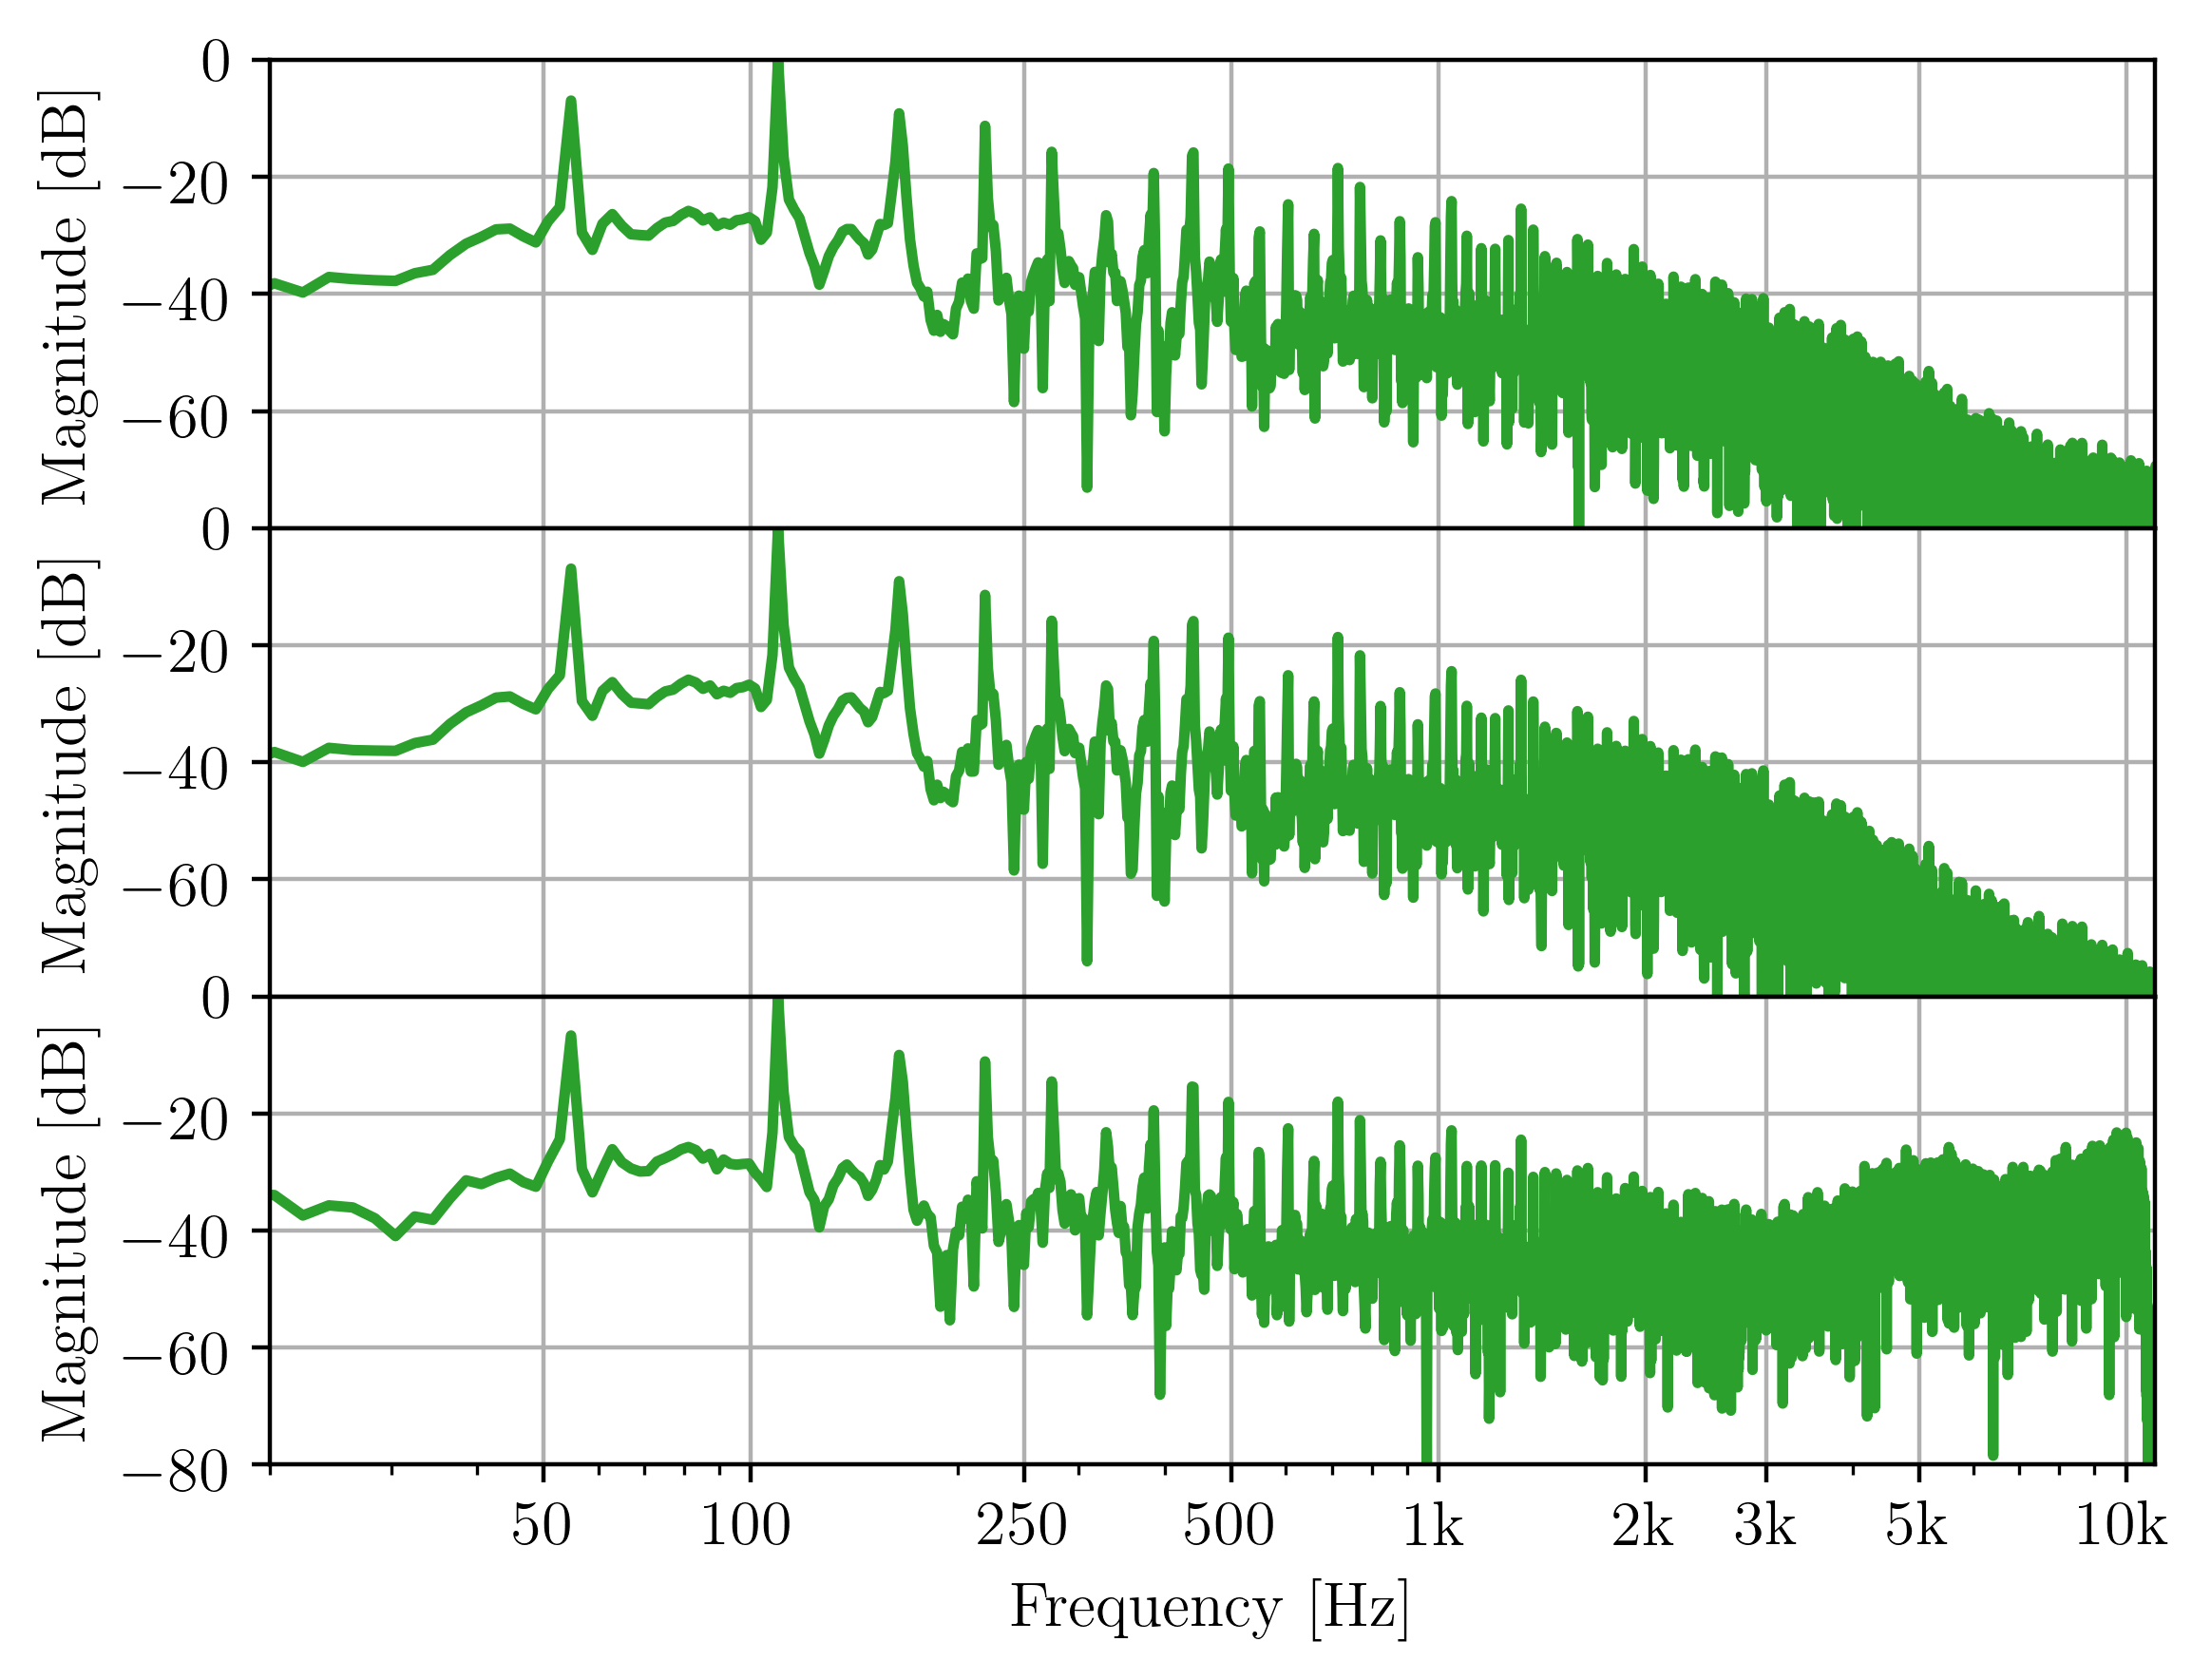
\includegraphics{figures/tikz/diode_clipper_aliasing/diode_clipper_aliasing.tex.png}
    \caption{Magnitude frequency spectrum of the A2 note played on the bass guitar. (Top) Target spectrum. (Middle) ODENet9(FE) output at \SI{192000}{Hz} sampling rate. (Bottom) ODENet9(FE) output at \SI{192000}{Hz} sampling rate. All spectra were normalized to the highest absolute value before the conversion to the decibel scale.}
    \label{fig:diode_clipper_aliasing}
\end{figure}

For \SI{22050}{Hz} test sampling rate (half of the training sampling rate), the lowest loss value was obtained for \ac{RINN}4. The second best result, \ac{LSTM}8, obtained the highest \ac{segSNR} and \ac{PEAQ} and sounds most accurately in casual listening. 

The output of \ac{STN} as well as all ODENet models contain high amount of noise. Moreover, ODENet100(FE) and ODENet9(IA) fall into self-oscillations, i.e., contain a constant high-frequency component even when the input signal is very quiet. Although the noise sounds unpleasantly, it is a sign that the networks learned the true derivative (or the residual in the case of \ac{STN}) contained in the data. The derivative networks probably output a correct value but given a larger time step without any additional tuning, the produced sound contains components beyond the Nyquist frequency, which cause aliasing in the output sound. 

Although the casually perceived quality of \ac{LSTM} is quite good, all produced outputs received equally low \ac{PEAQ}. It seems that models that were not informed about the time step significantly outperformed the informed ones. Thus, they are more suitable for processing at sampling rates lower than the training sampling rate.

For \SI{48000}{Hz} test sampling rate, again \ac{LSTM} outperformed other models in the analyzed metrics, yet all models had test loss value smaller than 1\%. In casual listening, there is not much difference between the model outputs despite the low \ac{PEAQ}.

For \SI{192000}{Hz} test sampling rate, the advantage of ODENet becomes clear with the largest model having the lowest loss value and the biggest \ac{segSNR} and \ac{PEAQ}. The smaller ODENet models obtained just slightly worse results, especially given their significantly smaller number of parameters. As could be expected, architectures that take the sampling rate into account during processing (\ac{STN}, ODENet) obtained lower loss value and significantly higher \ac{PEAQ} than the non-informed ones. The only exception is the low \ac{PEAQ} of ODENet9(IA), probably because of the clicks resulting from all-zero initialization at the beginning of each segment and subsequent concatenation. A slower but more accurate implicit solver obtained loss comparable to a hundred times larger architecture using an explicit scheme. However, all test loss values are below 1\% and \ac{segSNR} is relatively high.

The magnitude frequency spectrum of a sample output of ODENet9(FE) at different sampling rates can be seen in \Figure{fig:diode_clipper_aliasing}. At \SI{192000}{Hz} test sampling rate, the magnitude spectrum (middle) is indistinguishable from the target (top). However, at \SI{22050}{Hz} sampling rate (bottom), significant aliasing artifact can be observed above \SI{2500}{Hz}.

All in all, ODENet architectures proved their suitability for processing at sampling rates higher than the training sampling rate. It was possible even for the smallest considered parametrization (9 hidden units) and the simplest numerical scheme, i.e., the forward Euler. 

There was an advantage of the implicit solver over the explicit one in terms of the loss value but at the cost of doubled time needed to process the same amount of data, as indicated by the training time in \Table{tab:diode_clipper_models_data}. 

For the diode clipper model, it does not seem beneficial to increase the derivative network's capacity beyond the necessary minimum (here: 9 units in the hidden layers). As mentioned in the introduction to \Section{sec:diode_clipper_models}, this minimum was found by decreasing the hidden layers' size and observing the validation error. Networks with a hidden size smaller than 9 had validation error significantly higher than 3\%: a threshold regarded as perceptually significant \cite{Wright2020}.

%%%%%%%%%%%%%%%%%%%%%%%%%%%%%%%%%%%%%%%%%%%%%%%%%%%%%%%%%%%%%%%%%%%%%%%%%%%%%%%%%%%%%%%
\subsubsection{Convergence Speed}
%%%%%%%%%%%%%%%%%%%%%%%%%%%%%%%%%%%%%%%%%%%%%%%%%%%%%%%%%%%%%%%%%%%%%%%%%%%%%%%%%%%%%%%

\begin{figure}
    \centering
    \begin{tikzpicture}
    \begin{axis}[
        no markers,
        every axis plot/.append style={ultra thick},
        xmin = 0,
        xmax = 200,
        grid,
        xlabel = Epoch,
        ylabel = Validation Loss,
    ]
        \addplot[smooth,mark=none,color=red, dashed] table [x=Step, y=Value, col sep=comma] {figures/tikz/diode_clipper_validation_curves/run-forward_euler_July16_13-14-04_axel_ODENet2Hidden9-tag-Loss_validation.csv};
        \addplot[smooth,mark=none,color=blue] table [x=Step, y=Value, col sep=comma] {figures/tikz/diode_clipper_validation_curves/run-lstm_June30_13-57-49_axel-tag-Loss_validation.csv};
        \legend{ODENet9(FE), LSTM8};
    \end{axis}
\end{tikzpicture}

    \caption{Convergence curves of two diode clipper models.}
    \label{fig:diode_clipper_validation_curves}
\end{figure}

Looking at how the validation loss of ODENet and LSTM changes during training, as shown in \Figure{fig:diode_clipper_validation_curves}, one can observe that the former takes many more epochs to get below 1\% than the latter. This may be explained by the nature of the \ac{LSTM} architecture, where the constant-error carousel ensures that error gets propagated even for very long time lags \cite{Hochreiter1997}. Slow convergence can be seen as a disadvantage of the ODENet framework, slowing down the derivative network architecture exploration or hyperparameter search. Increasing the learning rate of the ODENet, for example, by using the one-cycle learning rate schedule, has proven itself beneficial but must be used with care; if the learning rate is too large, ODENet diverges.

%%%%%%%%%%%%%%%%%%%%%%%%%%%%%%%%%%%%%%%%%%%%%%%%%%%%%%%%%%%%%%%%%%%%%%%%%%%%%%%%%%%%%%%
\subsubsection{Comparison to Numerical Solvers}
%%%%%%%%%%%%%%%%%%%%%%%%%%%%%%%%%%%%%%%%%%%%%%%%%%%%%%%%%%%%%%%%%%%%%%%%%%%%%%%%%%%%%%%

To get a sense of how a learned derivative performs in comparison to the closed-form formula, a numerical solver was run on the diode clipper \ac{ODE} as presented in \Equation{eq:diode_clipper_equation} using the test set at \SI{44100}{Hz} sampling rate. To avoid aliasing, we oversampled the data before supplying it to the solver. The initial experiments showed, that scaling the input data by a factor of 20 significantly decreased the loss. After the solver completed the processing, its output was rescaled so as to minimize the \ac{ESR} as given by \Equation{eq:esr}. The loss function-informed scaling was supposed to compensate for the fact that the solver or the \ac{ODE} could not learn the proper scaling in a training phase as the \ac{ANN} models could and that scaling in itself should not determine the loss value of the solver's output. 

The results of solving the diode clipper \ac{ODE} with the \ac{BDF} solver at 8x sampling rate and with the \ac{RK}4 solver at 30x sampling rate are presented in \Table{tab:diode_clipper_ode_solvers}. These solvers are a part of Scipy library \cite{SciPy}. The metrics were computed with respect to the target of the test set used to evaluate the \ac{ANN} models.

\begin{table}[]
    \centering
    \begin{tabular}{@{}|l|c|c|@{}}
    \toprule
    Metric & \makecell{\ac{ODE} \acs{BDF}\\8x oversampling} & \makecell{\ac{ODE} \ac{RK}4\\30x oversampling} \\ \midrule
    Loss   & 0.52\% & 0.54\% \\
    segSNR & 16.2 & 16.2 \\
    ODG    & -3.2 & -3.3 \\ \bottomrule
\end{tabular}%

    \caption{Results of numerical solutions of the diode clipper \ac{ODE}.}
    \label{tab:diode_clipper_ode_solvers}
\end{table}

One can observe that the numerical solutions of the \ac{ODE} achieved less than 1\% of the test loss. At the same time they obtained much lower values of \ac{segSNR} and \ac{PEAQ} than the ODENet models from \Table{tab:diode_clipper_results}. Moreover, the data input to the ODENet did not need any oversampling, because having a non-aliased dataset significantly diminishes the chance of the derivative network learning an aliasing behavior. Thus, apart from not having to derive the \ac{ODE} and learning it from data instead, ODENet additionally does not need its input to be oversampled.

It needs to be stressed again, that data used to conduct the training and tests of the \acp{ANN} was synthesized using LTspice \cite{LTspice}. There is, however, no reason to doubt that the networks would perform equally well on discretized, measured data.

\newcommand{\subfigureWidth}{0.4\textwidth}
\newcommand{\subfigureScale}{0.8}

\begin{figure}
    \centering
    \begin{subfigure}{0.9\textwidth}
        \centering
        \scalebox{\subfigureScale}{% This file was created by tikzplotlib v0.9.9.
\begin{tikzpicture}

\begin{axis}[
colorbar,
colorbar style={ytick={-50,-25,-7.105427357601e-15,25,50,75},yticklabels={
  \(\displaystyle {\ensuremath{-}50}\),
  \(\displaystyle {\ensuremath{-}25}\),
  \(\displaystyle {0}\),
  \(\displaystyle {25}\),
  \(\displaystyle {50}\),
  \(\displaystyle {75}\)
},ylabel={}},
colormap/viridis,
point meta max=89.8890028498266,
point meta min=-59.9966700068274,
tick align=outside,
tick pos=left,
x grid style={white!69.0196078431373!black},
xlabel={$\text{Input}/20$},
xmin=-1, xmax=1,
xtick style={color=black},
xtick={-1,-0.5,0,0.5,1},
xticklabels={
  \(\displaystyle {\ensuremath{-}1.0}\),
  \(\displaystyle {\ensuremath{-}0.5}\),
  \(\displaystyle {0.0}\),
  \(\displaystyle {0.5}\),
  \(\displaystyle {1.0}\)
},
y grid style={white!69.0196078431373!black},
ylabel={Output},
ymin=-1, ymax=1,
ytick style={color=black},
ytick={-1,-0.5,0,0.5,1},
yticklabels={
  \(\displaystyle {\ensuremath{-}1.0}\),
  \(\displaystyle {\ensuremath{-}0.5}\),
  \(\displaystyle {0.0}\),
  \(\displaystyle {0.5}\),
  \(\displaystyle {1.0}\)
}
]
\addplot graphics [includegraphics cmd=\pgfimage,xmin=-1, xmax=1, ymin=-1, ymax=1] {figures/tikz/diode_clipper_derivative_visualization/analytical_derivative.tikz-000.png};
\end{axis}

\end{tikzpicture}
}
        \caption{After \Equation{eq:diode_clipper_equation}. Every magnitude $m$ is transformed to $10 \log_{10}(m)$.}
    \end{subfigure}
    \begin{subfigure}{0.9\textwidth}
        \centering
        \scalebox{\subfigureScale}{% This file was created by tikzplotlib v0.9.9.
\begin{tikzpicture}

\begin{axis}[
colorbar,
colorbar style={ytick={50000,100000,150000},yticklabels={
  \(\displaystyle {50000}\),
  \(\displaystyle {100000}\),
  \(\displaystyle {150000}\)
},ylabel={}},
colormap/viridis,
point meta max=154563.40625,
point meta min=0.0351317226886749,
tick align=outside,
tick pos=left,
x grid style={white!69.0196078431373!black},
xlabel={Input},
xmin=-1, xmax=1,
xtick style={color=black},
xtick={-1,-0.5,0,0.5,1},
xticklabels={
  \(\displaystyle {\ensuremath{-}1.0}\),
  \(\displaystyle {\ensuremath{-}0.5}\),
  \(\displaystyle {0.0}\),
  \(\displaystyle {0.5}\),
  \(\displaystyle {1.0}\)
},
y grid style={white!69.0196078431373!black},
ylabel={Output},
ymin=-1, ymax=1,
ytick style={color=black},
ytick={-1,-0.5,0,0.5,1},
yticklabels={
  \(\displaystyle {\ensuremath{-}1.0}\),
  \(\displaystyle {\ensuremath{-}0.5}\),
  \(\displaystyle {0.0}\),
  \(\displaystyle {0.5}\),
  \(\displaystyle {1.0}\)
}
]
\addplot graphics [includegraphics cmd=\pgfimage,xmin=-1, xmax=1, ymin=-1, ymax=1] {figures/tikz/diode_clipper_derivative_visualization/FE100-ode_derivative-000.png};
\end{axis}

\end{tikzpicture}
}
        \caption{ODENet100(FE)}
    \end{subfigure}
    \begin{subfigure}{\subfigureWidth}
        \scalebox{0.75}{% This file was created by tikzplotlib v0.9.9.
\begin{tikzpicture}

\begin{axis}[
% colorbar,
% colorbar style={ytick={20000,40000,60000,80000,100000},yticklabels={
%   \(\displaystyle {20000}\),
%   \(\displaystyle {40000}\),
%   \(\displaystyle {60000}\),
%   \(\displaystyle {80000}\),
%   \(\displaystyle {100000}\)
% },ylabel={}},
% colormap/viridis,
point meta max=106742.0625,
point meta min=0.010339617729187,
tick align=outside,
tick pos=left,
x grid style={white!69.0196078431373!black},
xlabel={Input},
xmin=-1, xmax=1,
xtick style={color=black},
xtick={-1,-0.5,0,0.5,1},
xticklabels={
  \(\displaystyle {\ensuremath{-}1.0}\),
  \(\displaystyle {\ensuremath{-}0.5}\),
  \(\displaystyle {0.0}\),
  \(\displaystyle {0.5}\),
  \(\displaystyle {1.0}\)
},
y grid style={white!69.0196078431373!black},
ylabel={Output},
ymin=-1, ymax=1,
ytick style={color=black},
ytick={-1,-0.5,0,0.5,1},
yticklabels={
  \(\displaystyle {\ensuremath{-}1.0}\),
  \(\displaystyle {\ensuremath{-}0.5}\),
  \(\displaystyle {0.0}\),
  \(\displaystyle {0.5}\),
  \(\displaystyle {1.0}\)
}
]
\addplot graphics [includegraphics cmd=\pgfimage,xmin=-1, xmax=1, ymin=-1, ymax=1] {figures/tikz/diode_clipper_derivative_visualization/FE9-ode_derivative-000.png};
\end{axis}

\end{tikzpicture}
}
        \caption{ODENet9(FE)}
    \end{subfigure}
    \begin{subfigure}{\subfigureWidth}
        \scalebox{0.76}{% This file was created by tikzplotlib v0.9.9.
\begin{tikzpicture}

\begin{axis}[
colorbar,
colorbar style={ytick={50000,100000,150000,200000,250000},yticklabels={
  \(\displaystyle {50000}\),
  \(\displaystyle {100000}\),
  \(\displaystyle {150000}\),
  \(\displaystyle {200000}\),
  \(\displaystyle {250000}\)
},ylabel={}},
colormap/viridis,
point meta max=273656.71875,
point meta min=0.00042724609375,
tick align=outside,
tick pos=left,
x grid style={white!69.0196078431373!black},
xlabel={Input},
xmin=-1, xmax=1,
xtick style={color=black},
% xtick={-1,-0.5,0,0.5,1},
xtick={-0.5,0,0.5,1},
xticklabels={
  % \(\displaystyle {\ensuremath{-}1.0}\),
  \(\displaystyle {\ensuremath{-}0.5}\),
  \(\displaystyle {0.0}\),
  \(\displaystyle {0.5}\),
  \(\displaystyle {1.0}\)
},
% y grid style={white!69.0196078431373!black},
% ylabel={Output},
ymin=-1, ymax=1,
% ytick style={color=black},
% ytick={-1,-0.5,0,0.5,1},
ytick=\empty,
% yticklabels={
  % \(\displaystyle {\ensuremath{-}1.0}\),
  % \(\displaystyle {\ensuremath{-}0.5}\),
  % \(\displaystyle {0.0}\),
  % \(\displaystyle {0.5}\),
  % \(\displaystyle {1.0}\)
% }
]
\addplot graphics [includegraphics cmd=\pgfimage,xmin=-1, xmax=1, ymin=-1, ymax=1] {figures/tikz/diode_clipper_derivative_visualization/IA-ode_derivative-000.png};
\end{axis}

\end{tikzpicture}
}
        \caption{ODENet9(IA)}
    \end{subfigure}
    \caption{Magnitude of the derivative (analytical or learned) for given input and output signal values of the diode clipper.}
    \label{fig:diode_clipper_derivative_visualizations}
\end{figure}

In \Figure{fig:diode_clipper_derivative_visualizations} the derivative function given by \Equation{eq:diode_clipper_equation} and learned by ODENet100(FE), ODENet9(FE), and ODENet9(IA)  are visualized. The $x$-axis spans the input signal range, the $y$-axis spans the output signal range, and with color the magnitude of the derivative function in this two-dimensional space is indicated. Additionally, to enable at all an inspection of the analytical derivative, its magnitude $m$ was transformed to $10 \log_{10}(m)$. While there is not much difference between the derivative functions learned by the derivative networks, they are significantly different from the analytical form. This difference probably comes from time discretization of the training data, i.e., finite sampling rate. Additionally, the obtained results are on a par with the visualizations shown in \cite{Parker2019}.
